\subsection{Support Vector Machines for Linearly Separable Classes}
The following three chapters follow the support vector machine chapters 3.7 and 4.18 discussed in the book \emph{Pattern recognition} by Theodoridis and Koutroumbas \cite{PatternRecognition}.

I first discuss the Support Vector Machines in case of two linearly separable classes. Similarly to the previous section with linear classifiers, we design a hyperplane
\begin{equation}
g(\mathbf{x}) = \mathbf{w}^T \mathbf{x} + w_0 = 0
\end{equation}

\begin{figure}[here]
\centering
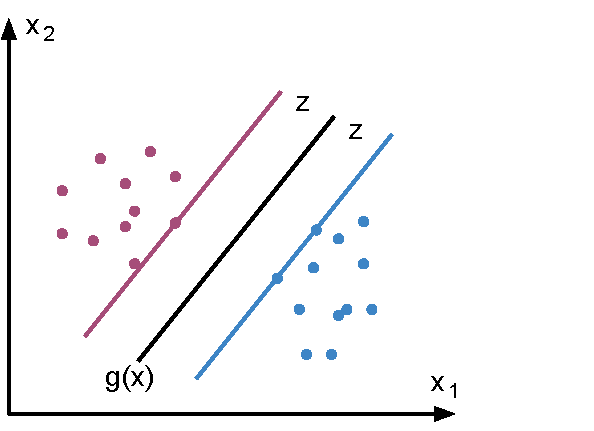
\includegraphics[scale=0.7]{images/svm_linear.pdf}
\caption{Maximum separating hyperplane between two linearly separable classes.}
\label{fig:svm_linear}
\end{figure}

When the hyperplane leaves maximal margins between the class instances and itself, the performance of classifier is optimal. This situation is depicted in Figure~\ref{fig:svm_linear}. Thus, we should maximize the margin $z$ which can be represented as $z = |g(\mathbf{x})| / ||\mathbf{w}||$. If we scale $\mathbf{w}$ and $w_0$ so that $g(\mathbf{x}) = 1$ for the class $w_1$ and $g(\mathbf{x}) = -1$ for the class $w_2$ on the points that are closest to the hyperplane, we have a margin of $2 / ||\mathbf{w}||$ and requirements
\begin{align}
\mathbf{w}^T \mathbf{x} + w_0 \ge 1, &\; \forall \mathbf{x} \in w_1 \\
\mathbf{w}^T \mathbf{x} + w_0 \le -1, &\; \forall \mathbf{x} \in w_2
\end{align}

We can form the problem as the following optimization problem
\begin{align}
\text{minimize} &\; J(\mathbf{w}, w_0) = \frac{1}{2} ||\mathbf{w}||^2 \\
\text{subject to} &\; y_i (\mathbf{w}^T \mathbf{x}_i + w_0) \ge 1, \; i = 1,2,...,N \label{eq:svm_linear_variables} 
\end{align}
where $y_1 = 1$ and $y_2 = -1$. The Karush-Kuhn-Tucker (KKT) conditions for this nonlinear quadratic optimization problem are
\begin{eqnarray} 
L_{\mathbf{w}}(\mathbf{w}, w_0, \mathbf{\lambda}) &=& \mathbf{0} \label{eq:KKT} \\
L_{w_0}(\mathbf{w}, w_0, \mathbf{\lambda}) &=& 0 \\
\lambda_i &\ge& 0, \; i = 1, 2, ..., N \\
\lambda_i [y_i (\mathbf{w}^T \mathbf{x}_i + w_0) - 1] &=& 0,
i = 1, 2, ..., N,
\end{eqnarray}
where $L(\mathbf{w}, w_0, \mathbf{\lambda})$ is the Lagrangian function
\begin{equation}
L(\mathbf{w}, w_0, \mathbf{\lambda}) = \frac{1}{2} \mathbf{w}^T \mathbf{w} - \sum_{i=1}^N \lambda_i [y_i (\mathbf{w}^T \mathbf{x}_i + w_0) - 1]
\end{equation}

Solving the first order differential equations in the KKT conditions yields a dual problem
\begin{eqnarray}
\text{maximize} &\;& L(\mathbf{w}, w_0, \lambda) \\
\text{subject to} &\;& \mathbf{w} = \sum_{i=1}^N \lambda_i y_i \mathbf{x}_i \\
&& \sum_{i=1}^N \lambda_i y_i = 0 \\
&& \mathbf{\lambda} \ge \mathbf{0}
\end{eqnarray}

By substituting the first two conditions into the Lagrangian $L$ we further get
\begin{eqnarray}
&\underset{\mathbf{\lambda}}{\operatorname{max}}& \left ( \sum_{i=1}^N \lambda_i - \frac{1}{2} \sum_{i, j} \lambda_i \lambda_j y_i y_j \mathbf{x}_i^T \mathbf{x}_j \right ) \label{eq:SVM_KKT_1} \\ 
&\text{subject to}& \sum_{i=1}^N \lambda_i y_i = 0 \label{eq:SVM_KKT_2} \\ 
&&\mathbf{\lambda} \ge 0 \label{eq:SVM_KKT_3}
\end{eqnarray}

As we can easily see, the function to be maximized does not depend on the dimensionality of the input space because it contains the input vectors in the form of a inner product. This allows us to easily generalize the method into non-separable classes by mapping them into a higher-dimensional space in the next sections.

The Support Vectors are the points $\mathbf{x}_i$ for which the Lagrangian multiplier $\lambda_i$ is not zero and which lie on one of the hyperplanes $\mathbf{w}^T \mathbf{x} + w_0 = \pm 1$. The optimal hyperplane of SVM is unique because the cost function in equation~\ref{eq:KKT} is strictly convex.


\subsection{Support Vector Machines for Linearly Non-separable Classes}
Now we turn to the case of classes that cannot be separated with a linear hyperplane. In this case we introduce slack variables $\xi_i \ge 0$ that allow some points to fall on the wrong side of the hyperplane. Now the equation~\ref{eq:svm_linear_variables} is replaced with
\begin{equation}
y_i [\mathbf{w}^T \mathbf{x} + w_0] \ge 1 - \xi_i,
\end{equation}  
where the value of $\xi_i$ defines the type of the point as follows:
\begin{enumerate}
\item $\xi_i = 0$ $\Rightarrow$ Point is classified correctly.
\item $0 < \xi_i \le 1$ $\Rightarrow$ Point is classified correctly but it is on the wrong side of the margin.
\item $\xi_i > 1$ $\Rightarrow$ Point is misclassified.
\end{enumerate}

These three types are illustrated in figure~\ref{fig:svm_non_separable}. An yellow ring marks a point that is classified correctly but that is on the wrong side of the margin (type 2). A red square marks a point that is misclassified (type 3).  

\begin{figure}[here]
\centering
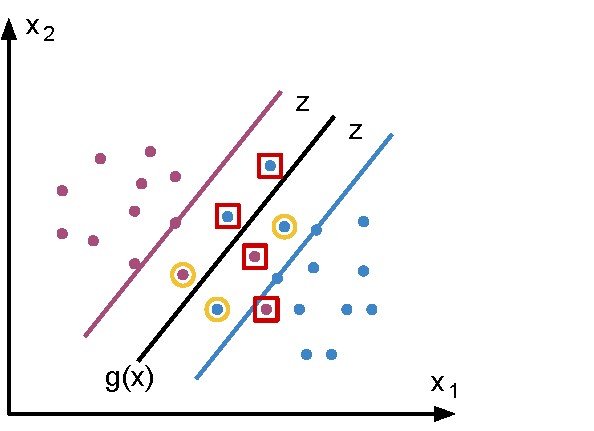
\includegraphics[scale=0.7]{images/svm_non_separable.pdf}
\caption{A separating hyperplane between two classes that are non-separable. A yellow ring marks a point that is classified correctly but that is on the wrong side of the margin. A red square marks a point that is misclassified.}
\label{fig:svm_non_separable}
\end{figure}

In this case our optimization problem can be stated as
\begin{align}
\text{minimize} &\; J(\mathbf{w}, w_0, \mathbf{\xi}) = \frac{1}{2} ||\mathbf{w}||^2 + C \sum_{i=1}^N I(\xi_i) \label{eq:SVM_C_parameter} \\
\text{subject to} &\; y_i [\mathbf{w}^T \mathbf{x}_i + w_0] \ge 1 - \xi_i, i = 1, 2, ..., N \\
& \xi_i \ge 0, i = 1, 2, ..., N,
\end{align}
where $I(\xi_i) = 1$ if $\xi_i > 0$ and $I(\xi_i) = 0$ if $\xi_i = 0$ and the parameter $C$ defines a trade-off between maximizing the margin and minimizing the number of misclassified points. Similarly to the previous section, we can build a dual problem that leads to the problem
\begin{align}
\underset{\mathbf{\lambda}}{\operatorname{max}} &\; \left ( \sum_{i=1}^N \lambda_i - \frac{1}{2} \sum_{i,j} \lambda_i \lambda_j y_i y_j \mathbf{x}_i^T \mathbf{x}_j \right ) \\
\text{subject to} &\; 0 \le \lambda_i \le C, i = 1, 2, ..., N \\
&\; \sum_{i=1}^N \lambda_i y_i = 0.
\end{align}

Again, the dimensionality of the input space disappears from the problem and the input vectors appear only as inner products. There is a shortcut for calculating these inner products with a kernel trick \cite{Jordan04}, which is described in the next section.

\subsection{Generalization of SVMs into Nonlinear Cases}
\begin{figure}[here]
\centering
\includegraphics[scale=0.7]{images/svm_mapping.pdf}
\caption{The main idea of Support Vector Machines. Classes are not linearly separable in the input space. They are mapped into a higher-dimensional space where a linear classifier can be formed. This classifier corresponds to a non-linear classifier in the original input space.}
\label{fig:svm_mapping}
\end{figure}


If the classes are not separable in the $l$-dimensional input space, we can find a mapping $\mathbf{x} \in \mathbb{R}^l \; \rightarrow \; \mathbf{y} \in \mathbb{R}^k$, where $k > l$. The choice of $k$ is done so that the original classes are linearly separable in the new, higher-dimensional space. This situation is depicted in Figure~\ref{fig:svm_mapping}. As mentioned in the previous chapters, our optimization problems contain input vector $x$ only as an inner product that is not altered by the mapping.

In order to present the Mercer's Theorem \cite{Jordan04} that relates the inner product to a kernel function, we need to explain some space related concepts. A Cauchy sequence is defined as a sequence $a_1, a_2, ...$ for which
\begin{equation}
\forall \epsilon \in \mathbb{R} \; \exists \; N > 0  \; s.t.  \; |a_m - a_n| < \epsilon, \; m, n > N
\end{equation}
In other words, the elements of the sequence become arbitrarily close as the sequence progresses. A complete space is a space where every Cauchy sequence converges to a point that is also contained within the space. A Hilbert space, in turn, is a generalization of Euclidean space into any finite or infinite number of dimensions. It is a complete vector space that has inner product defined for measuring lengths and angles. \cite{duchateau02}

Mercer's Theorem states that for each mapping $\mathbf{x} \rightarrow \mathbf{\phi}(\mathbf{x}) \in H$, where $H$ is a Hilbert Space, we have a kernel function $K(\mathbf{x}, \mathbf{y})$ that is equivalent for the inner product:
\begin{equation}
\left \langle \mathbf{\phi}(\mathbf{x}), \mathbf{\phi}(\mathbf{y}) \right \rangle = K(\mathbf{x}, \mathbf{y}).
\end{equation}

The kernel function must have the following properties
\begin{align}
\int_S \int_S K(\mathbf{x}, \mathbf{y})g(\mathbf{x})g(\mathbf{y})d\mathbf{x}d\mathbf{y} &\ge 0 \\ 
\int_S g(\mathbf{x})^2 d\mathbf{x} &< +\infty, \; \forall g(\mathbf{x}), \mathbf{x} \in S, 
\end{align}
where $S \subset \mathbb{R}^l$. The opposite is also true: for any Kernel function satisfying the conditions above there is a Hilbert space where the Kernel function is equivalent for the inner product. The problem is now how to find the mapping $\phi$ when we have selected the Kernel function.

Now we can replace the inner product in Equation~\ref{eq:SVM_KKT_1} with the Kernel function to get the optimization problem
\begin{align}
\underset{\mathbf{\lambda}}{\operatorname{max}} &\left ( \sum_i \lambda_i - \frac{1}{2} \sum_{i,j} \lambda_i \lambda_j y_i y_j K(\mathbf{x}_i, \mathbf{x}_j) \right ) \label{eq:SVM_final_problem} \\
\text{subject to} &\; 0 \le \lambda_i \le C, \; i = 1, 2, ..., N \\
&\; \sum_i \lambda_i y_i = 0.
\end{align}

The resulting non-linear classifier is then
\begin{equation}
g(\mathbf{x}) = \sum_{i=1}^{N_s} \lambda_i y_i K(\mathbf{x}_i, \mathbf{x}) + w_0 \begin{cases}
> 0, \; \Rightarrow \mathbf{x} \in w_1 \\
< 0, \; \Rightarrow \mathbf{x} \in w_2,
\end{cases} \label{eq:SVM_classifier}, 
\end{equation}
which is shown in Figure~\ref{fig:svm_network}. Input vectors enter the network from the left. Then, inner products are calculated in middle nodes, the number of which is N, the number of support vectors. An output node sums the components up and outputs a single real number that determines the result of the classification according to equation~\ref{eq:SVM_classifier}.


\begin{figure}[here]
\centering
\includegraphics[scale=0.7]{images/svm_network.pdf}
\caption{SVM classifier as a network. Input vectors enter the network from the left. Kernel functions calculate inner products in the middle nodes. Output node combines sums the components up and outputs a single real number.}
\label{fig:svm_network}
\end{figure}



\subsection{Using SVM for Time Series Analysis}
Before we can use our SVM classifier, we have to choose an appropriate kernel function $K(\mathbf{x}, \mathbf{y})$ for classifying wavelet based feature vectors. In literature one of the most used kernels is the Gaussian kernel \cite{Zhang04}, which is of the form
\begin{equation}
K(\mathbf{x}, \mathbf{y}) = \exp{\frac{||\mathbf{x} - \mathbf{y}||^2}{2\gamma^2}}, \label{eq:RBF_kernel},
\end{equation}
where $\beta > 0$ is a parameter chosen by the user. Gaussian kernel belongs to a family of functions called radial basis functions (RBF) whose value depends only on the distance between two points \cite{Scholkopf97}
\begin{equation}
f(\mathbf{x}, \mathbf{y}) = f(||\mathbf{x} - \mathbf{y}||)
\end{equation}

If we assume that the time series is generated by an AR(1)-process 
\begin{align}
x_T = g(x_{T-1}, ..., x_{T-k}) + \mu,
\end{align}
it can be shown that an ellipsoid with mean equal to the mean of the time series and variance equal to $\mu$ contains most of the data. The variable $\mu$ is a Gaussian noise component. Consequently, similar time windows are close to each other in the sense of Euclidean Distance. This makes RBF Kernels promising for time series analysis. \cite{Ruping01}

Another possibility is Polynomial Kernel that is of the form
\begin{equation}
K(\mathbf{x}, \mathbf{y}) = (\mathbf{x}^T \mathbf{y} + c)^d,
\end{equation}
which gives the Linear Kernel as a special case when $d = 1$. \cite{Scholkopf97}

Subsequence Kernels look for informative subsequences that are similar in dependent time windows. In this case the Kernel function becomes
\begin{equation}
K(\mathbf{x}, \mathbf{y}) = \sum_{s_x, s_y} K (s_x, s_y),
\end{equation}
where $s_x$ and $s_y$ are subsequences of x and y. There are $\binom{n}{k}^2$ possible combinations for time series of length $n$ and subsequence of length $k$, so one must use another algorithm for selecting the optimal subsequences. \cite{Ruping01}

In thesis I use Gaussian RBF Kernels because of their widespread use and good applicability to time series analysis. Ruping \cite{Ruping01} compared Linear, RBF, Fourier, Subsequence and Hidden Markov Model Kernels and came into conclusion that RBF Kernels perform very well on time series learning tasks. However, he recommends to investigate other possibilities in very specialized applications.

A well defined kernel function increases the performance of the SVM greatly and thus Kernel selection is an important part of SVM development \cite{Fong04}. In the case of RBF Kernels we must choose the value of $\gamma$ in \ref{eq:RBF_kernel}. From now on I try to find an optimal value for $\sigma$, which then defines the $\gamma$ from $\gamma = 1 / 2\sigma^2$. The value of $\sigma$ should be chosen so that it minimizes the error
\begin{equation}
E(\sigma) = \sum_{i=1}^N \left | g(\mathbf{x}_i, \sigma) - y_i \right |^2 \label{eq:SVM_error}
\end{equation}

A related theorem states that for a Support Vector Classifier (SVC) there exists a range $[\sigma_A, \sigma_B]$ for which
\begin{align}
&\forall \; \epsilon > 0 \;\; \text{and} \;\; \forall \; \sigma_1, \sigma_2 \in [\sigma_A, \sigma_B] \\
& \left | \sum_{i=1}^N \left | g(\mathbf{x}_i, \sigma_1) - y_i \right | - \sum_{i=1}^N \left | g(\mathbf{x}_i, \sigma_2) - y_i \right | \right | < \epsilon,
\end{align}
where $g(\mathbf{x}_i, \sigma_i)$ is the discriminant function from Equation~\ref{eq:SVM_classifier} and $y_i$ is the desired output ($\pm 1$) \cite{Wenjian08}. In other words, there is a range for $\sigma$ where the Gaussian Kernel's generalization performance is stable. 

To summarize our parameter estimation problem, we have two unknown parameters, Gaussian Kernel parameter $\gamma$ and SVM weighting parameter $C$ from \ref{eq:SVM_C_parameter}. Now there are two ways to find the optimal values for the parameters: gradient search and grid search. Staelin \cite{Staelin03} compared these two methods and came into the conclusion that they both achieve similar results in terms of accuracy. The only difference is clearly the computational cost that is much greater for the grid search. 

To keep things simple, only the grid search is employed in this thesis. The grid is formed as follows
\begin{align}
\ln{\gamma} &\in \left \{ \ln{\gamma_0} - a_0, \ln{\gamma_0} - a_0 + 1, ..., \ln{\gamma_0}, ..., \ln{\gamma_0} + a_0 \right \} \label{eq:svm_gamma} \\
\ln{C} &\in \left \{ 0, 1, ..., C_0 \right \}, \label{eq:svm_c}
\end{align}
where the parameters $\gamma_0$ and $C_0$ have to be chosen. Jaakkola's heuristics \cite{Jaakkola99} give us a initial guess for $\gamma_0$. Let $S$ be our training set. Then, from the set
\begin{equation}
G = \left \{ \lVert \mathbf{x}_i - \mathbf{x}_j \rVert \; | \; (\mathbf{x}_i, y_i), (\mathbf{x}_j, y_j) \in S, y_i \ne y_j \right \}
\end{equation}
we can compute
\begin{equation}
\sigma_0 = \sigma_{Jaakkola} = \operatorname{median}(G)
\end{equation}
and finally $\gamma_0 = 1 / \sigma_0^2$. The parameters $a_0$ and $C_0$ are chosen in the implementation chapter.

%K-fold Cross-Validation (K-CV) can be used to choose the optimal values for $\gamma$ and $C$ from the grid. First, we divide our training set $S$ randomly into $K$ subsets $S_1, ..., S_K$ so that the subsets are approximately of the same size. Let $S_{-i} = \bigcup_{j=1,...,K, j \ne i} S_i$ be the union of the subsets other than $S_i$ \cite{ChihWei10}. 

%For each ($\gamma$, $C$) pair we solve \ref{eq:SVM_final_problem} using data from $S_i$ to get the classifier $g(\mathbf{x})$. Then, we calculate the validation error \ref{eq:SVM_error} with data from $S_{-i}$. We repeat this for each $i$ and calculate the average error. The ($\gamma$, $C$) pair with the lowest average error is chosen for our model \cite{ChihWei10}.

